\chapter{Firebase}

\section{Architektur}

\subsection{Lösungsstrategie}

beschreibe cloud-serivces und tools, die genutzt werden

wie werden die NFAs erfüllt

\subsection{Bausteinsicht}

\subsection{Laufzeitsicht}

\subsubsection{Auflisten, Aktualisieren und Löschen eines Videos}

\begin{figure}
  \centering
  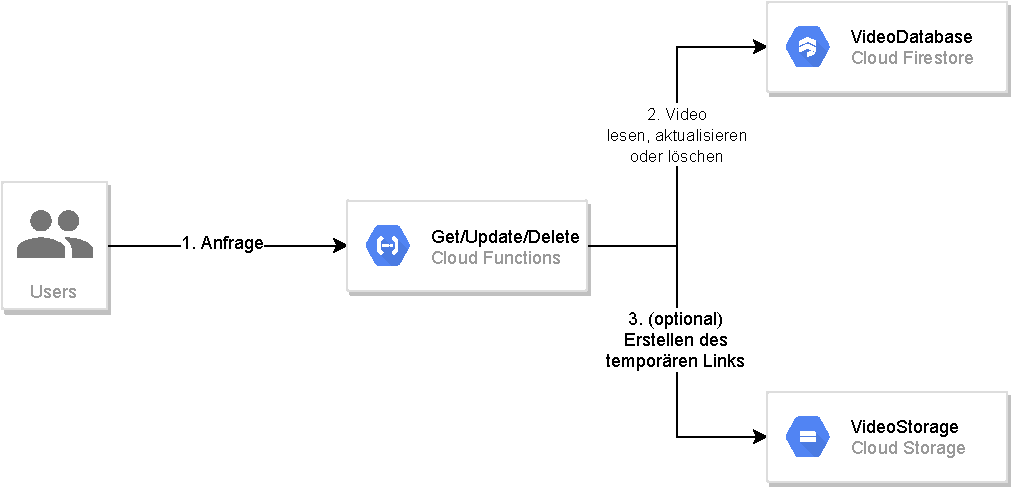
\includegraphics[width=1\columnwidth]{6_firebase/laufzeitsicht_1.pdf}
  \caption{Firebase - Laufzeitsicht - Lesen, Aktualisieren und Löschen eines Videos}
  \label{Firebase:laufzeitsicht1}
\end{figure}

\begin{figure}
  \centering
  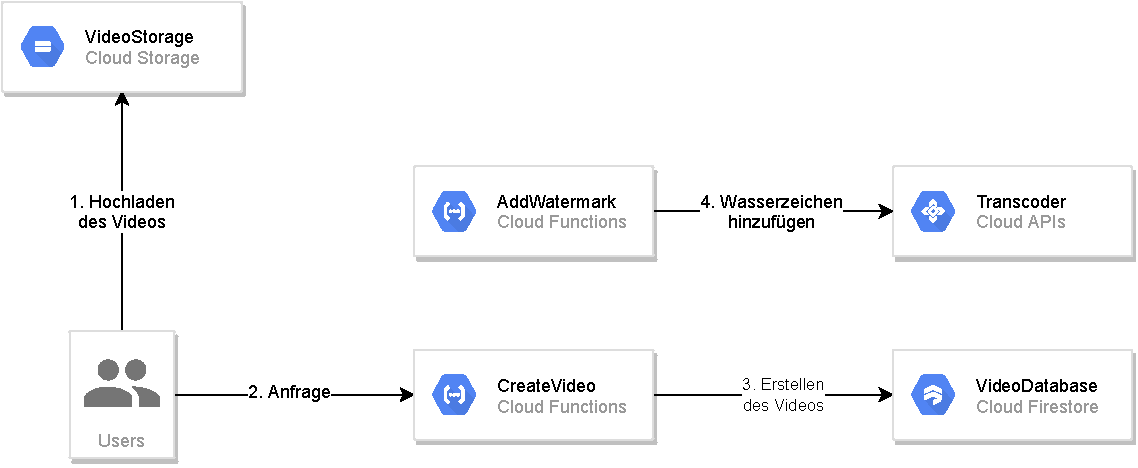
\includegraphics[width=1\columnwidth]{6_firebase/laufzeitsicht_2.pdf}
  \caption{Firebase - Laufzeitsicht - Erstellen eines Videos}
  \label{Firebase:laufzeitsicht2}
\end{figure}


Ablauf:
- Functions: update, delete
- 1. Call auf Function
- 2. Call auf Firestore von Function

- 3. Call auf Firebase Storage für presignedLink

- Besonderheiten beim Lesen
  - Search

- Besonderheiten bei Permissions (?)
  - prüfen, ob admin rolle oder ob owner, aber alles in separater DB gespeichert, nicht wie bei Cognito

\subsubsection{Erstellen eines Videos}

Functions:
- AddWaterMarkToVideo
- createVideo

0. Upload in firestore storage
1. Call to createVideo
2. Create video in firebase (with raw link to firestore)
3. Firestore Trigger executes on Create video/{docId}
4. Calls video-transcoder to add watermark, put in storage and put the new link in Firestore again


\subsection{Verteilungssicht}

\section{Implementierung}

todo